\documentclass[11pt, a4paper, oneside ]{article}
\usepackage{amsmath}
\usepackage{graphicx}
\usepackage{tabularx}
\usepackage{epstopdf}
\usepackage{float}
\usepackage{listings}
\usepackage{appendix}
\usepackage{fullpage}
\usepackage{caption}
\usepackage{gensymb}
\usepackage{url}
\usepackage{bold-extra}
\usepackage{siunitx}
\setlength{\parskip}{1em}
\lstset{
    basicstyle=\ttfamily
}
\author{Mark Stringer}
\title{\bf{Operation and Performance of the JSNS2 Driver System}}
\begin{document}
\pagenumbering{arabic}
\maketitle
\begin{abstract}
This report describes the operation of the JSNS2 driver system as well as the performance of one of the driver boards.
\end{abstract}

\section{Introduction}
This report describes the basic layout of the control box of the JSNS2 pulser system. Python commands to pulse the box are shown. In order to perform PMT timing calibrations the pulser system needs to be able to pulse at an intensity of \SI{e3}{photons } per pulse this report also presents the methodology and results of a study to confirm the driver can achieve this intensity when using both \SI{355}{nm} and \SI{420}{nm} LEDs.

\section{Operating the Control Box}

The control box for the JSNS2 driver system is shown in Figures~\ref{fig:boxFront} and~\ref{fig:boxBack}. A raspberry pi computer is situated within the control box. To operate the box you need to ssh into the raspberry pi using \texttt{ssh pi@139.184.130.87}. The IP address is currently fixed, the MAC address of the raspberry pi ethernet port is \texttt{b8:27:eb:ef:45:ee}.

\begin{figure}[H]
    \centering
    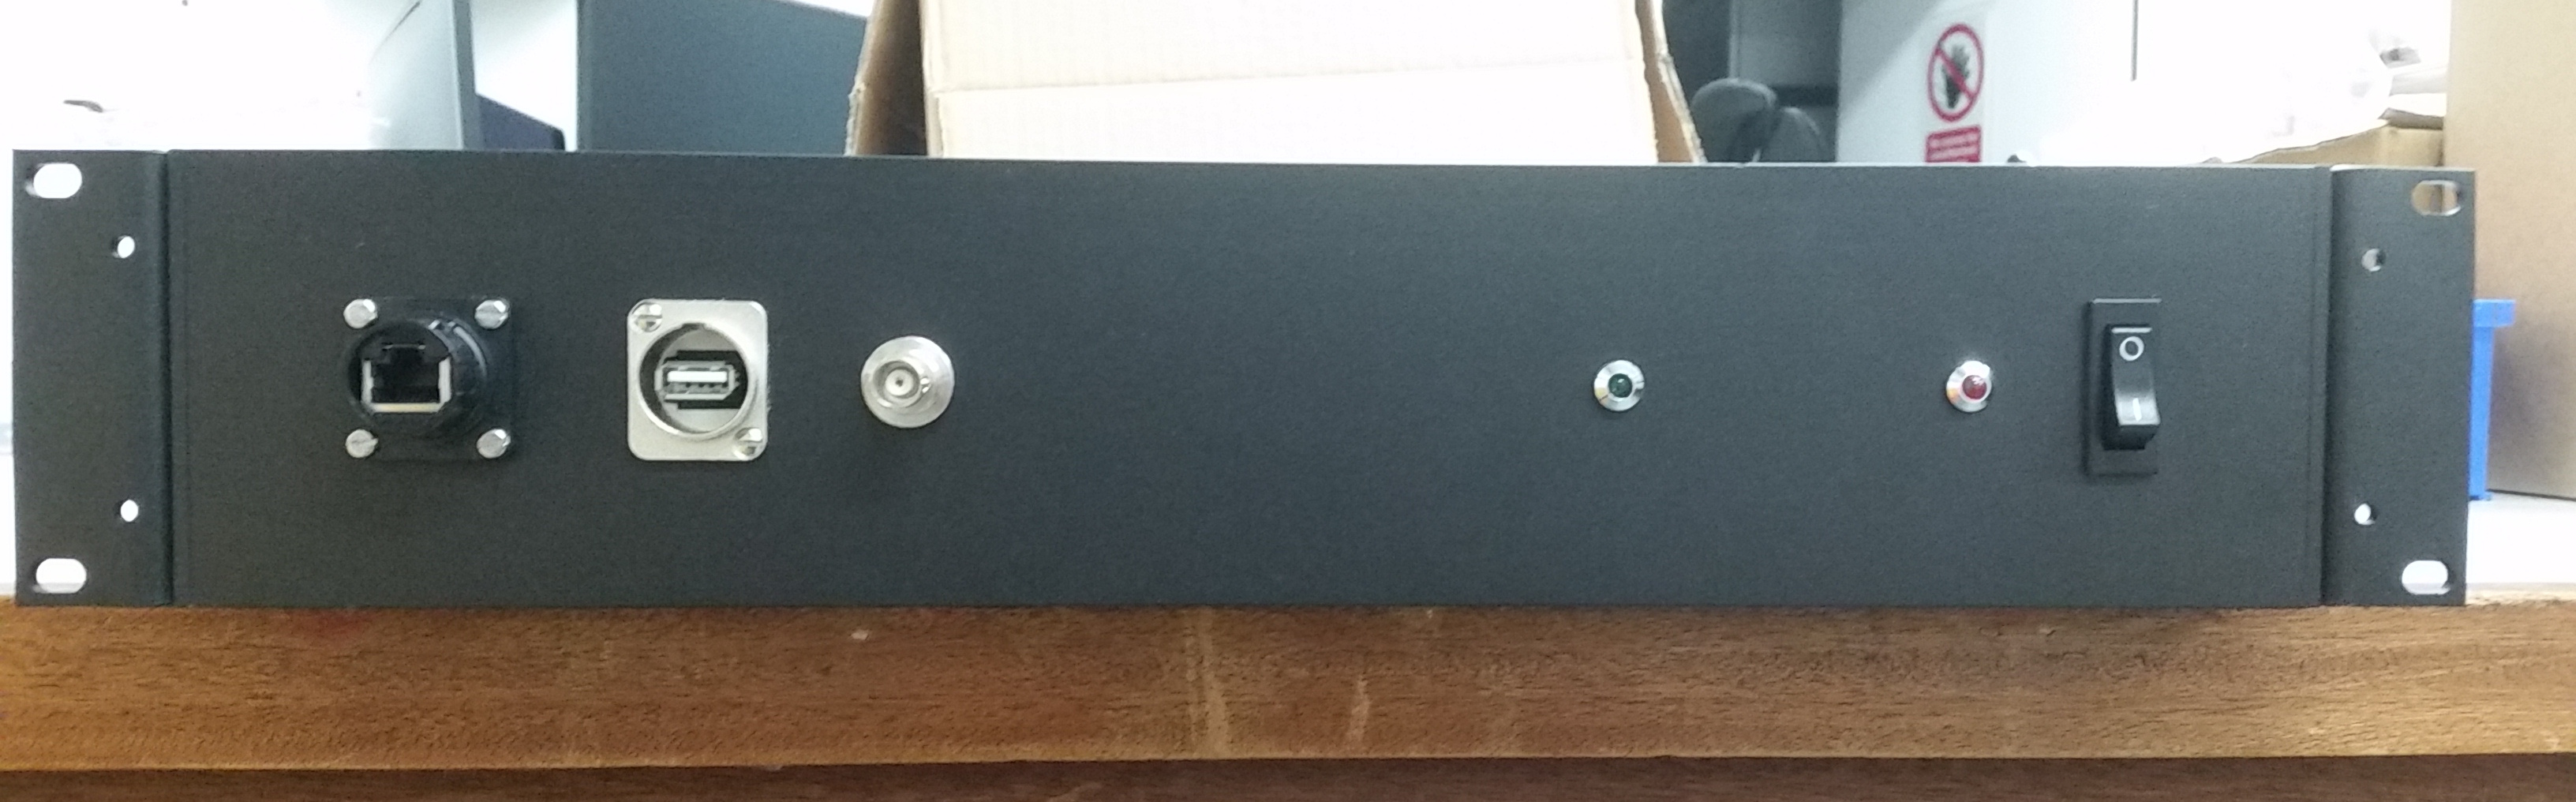
\includegraphics[width=0.8\textwidth]{figures/BoxFront.jpg}
    \caption{The front of the JSNS2 control box. From left to right the ports are: Ethernet for ssh access to the raspberry pi, USB access to the raspberry pi, Trigger out via BNC, Pulsing LED, Power LED, Power Switch.}
    \label{fig:boxFront}
\end{figure}

\begin{figure}[H]
    \centering
    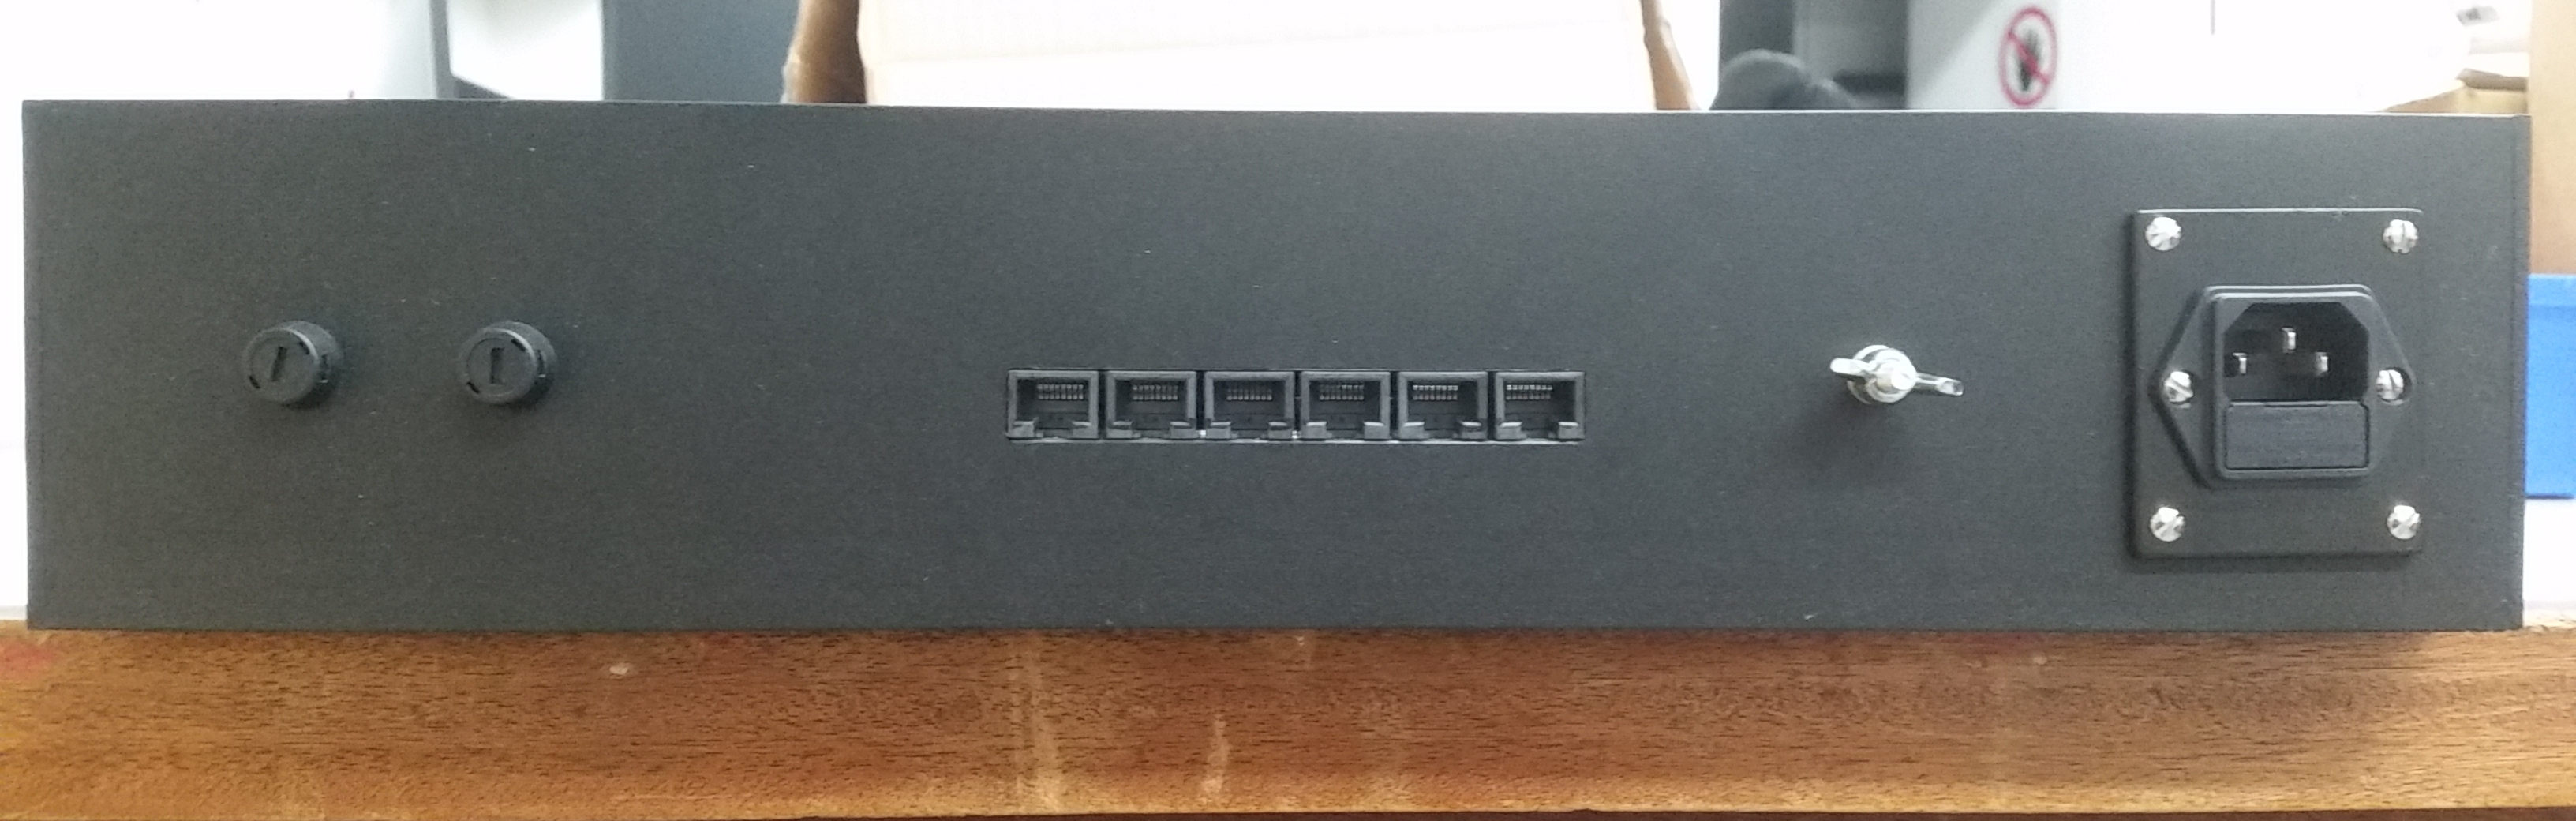
\includegraphics[width=0.8\textwidth]{figures/BoxBack.jpg}
    \caption{The back of the JSNS2 control box the ports from left to right fuse ports, ethernet ports for drivers, power socket}
    \label{fig:boxBack}
\end{figure}

\noindent The control scripts for the driver board are located in the folder: \newline\newline \texttt{/home/pi/JSNS2PulserControl/ControlSoftware/} \newline
\newline
\noindent The two scripts to control the driver boards are:
\newline
\newline
\texttt{\textbf{test\_run.py}} - Script to pulse the driver for a set number of pulses
\newline
\newline
\texttt{\textbf{test\_continuous.py}} - Script to pulse the driver for a set number of pulses
\newline
\newline
Both scripts take the following arguments:
\newline
\newline
\texttt{\textbf{-c}} - The channel to pulse \newline
\texttt{\textbf{-p}} - The pulse height for the driver board, this controls the intensity of each LED pulse. (Ranges from 0 to 16384)\newline
\texttt{\textbf{-d}} - The delay between pulses in milliseconds \newline
\newline
The \texttt{\textbf{test\_run.py}} script takes on additional parameter:
\newline
\newline
\texttt{\textbf{-n}} - Number of pulses\newline
\newline
\newline
The number of pulses must be a multiple of 1000.

\section{Performance of a single Driver Board}

The performance of a single driver board was quantified using a Thorlabs PM100USB optical power meter~\cite{PowermeterDataSheet} and a Hamamatsu H10721-210 desktop PMT~\cite{PMTDataSheet}. The initial calibration took place using the power meter, when the intensity of the pulse was reduced below the sensitivity of the power meter a PMT was used in conjunction with an oscilloscope to measure the intensity. The power meter is used to calibrate the gain of the PMT. During all measurements using the PMT and the power meter the driver is pulsed at 10 kHz. Two LED wavelengths were measured 420 nm and 355 nm.

\subsection{Measuring the intensity of the LED using the power meter}
Figure~\ref{fig:powerMeterSetup} shows the experimental setup of measuring the light output of the LED using the power meter. Both the power meter and the driver are located within the dark box, the end of the led is placed next to the face of the power meter sensor, and held in place using tape. 

\begin{figure}[H]
    \centering
    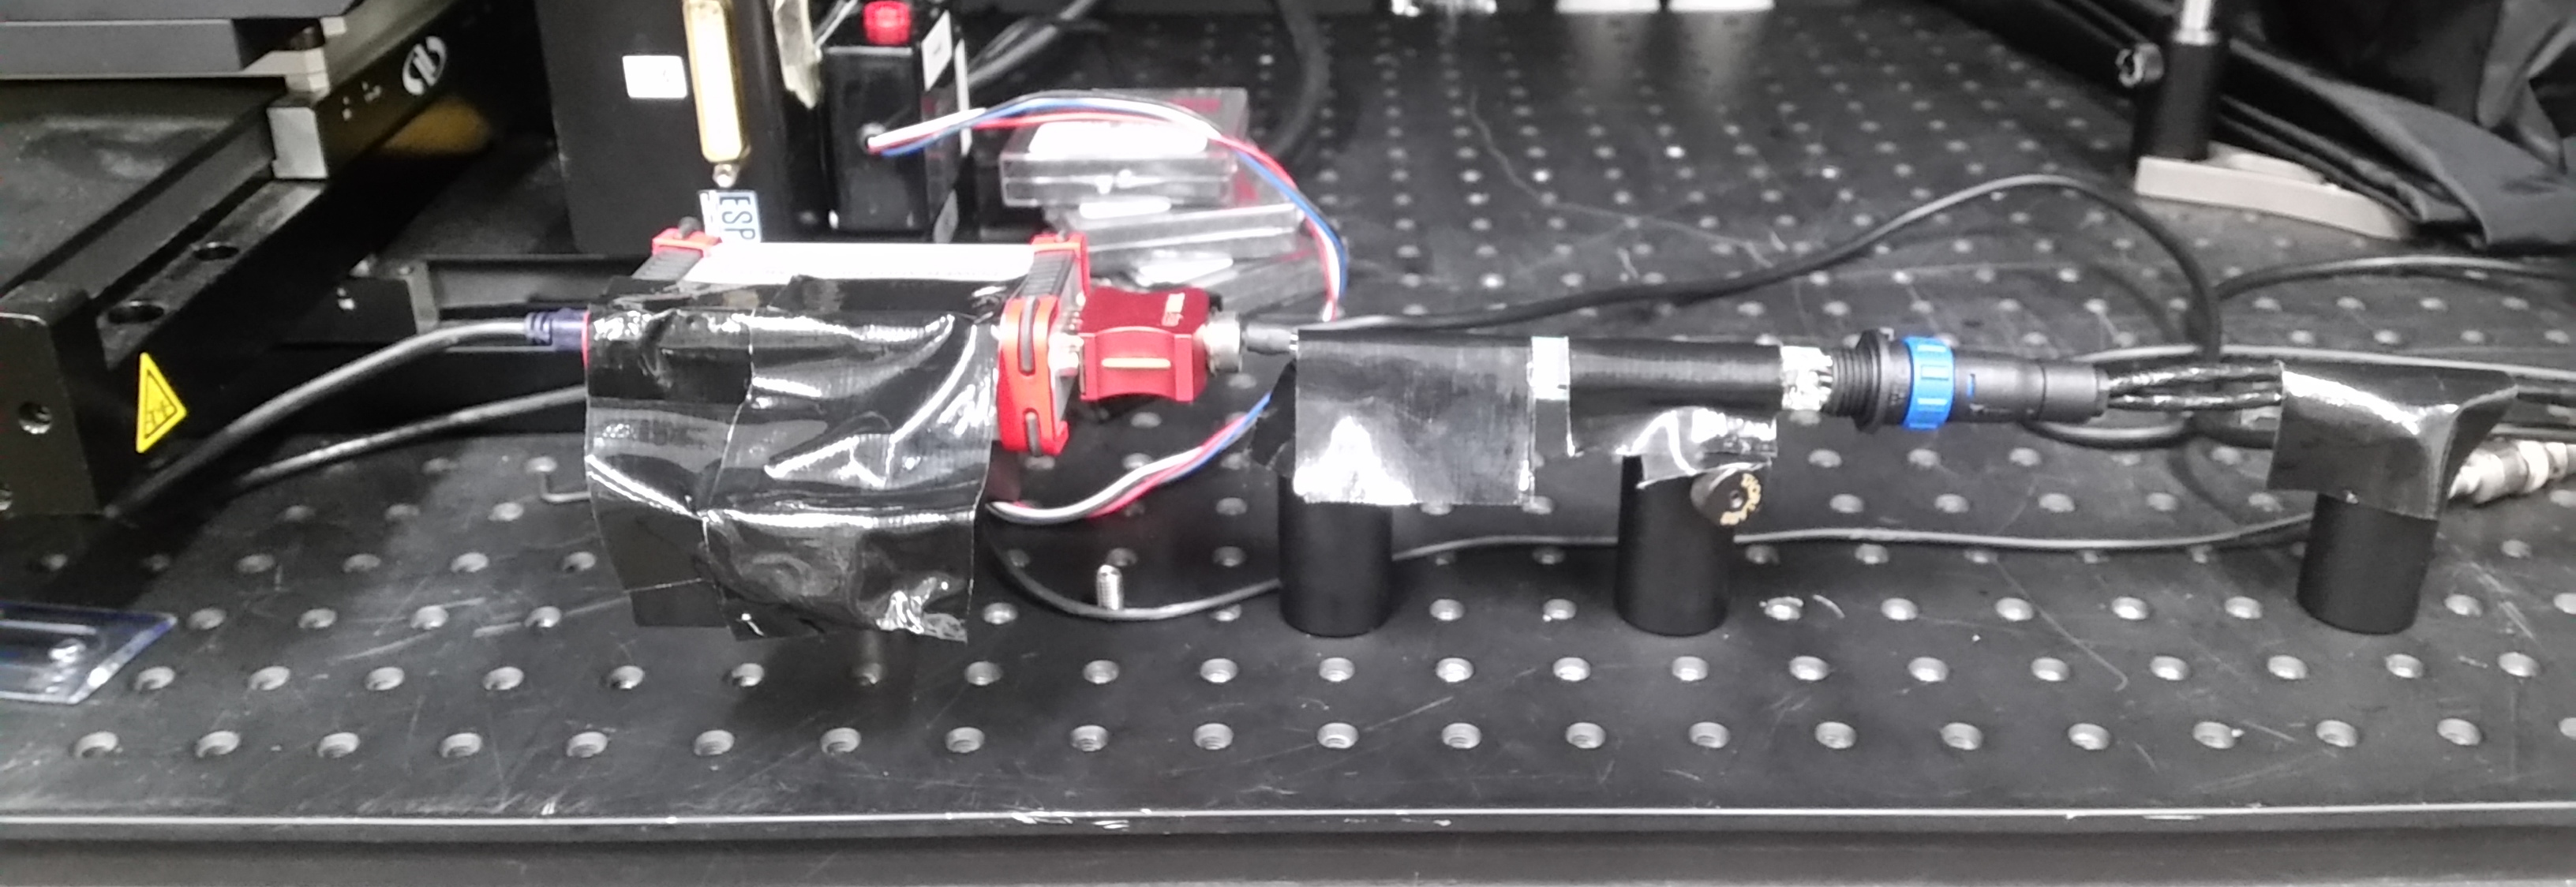
\includegraphics[width=\textwidth]{figures/PowerMeterSetup.jpg}
    \caption{The setup for measuring the intensity using the power meter.}
    \label{fig:powerMeterSetup}
\end{figure}

The power meter measures the power output in Watts. This is converted to the number of photons using Eq.~\ref{eq:photonsPowerMeter}. $E$ is the power output measured by the power meter $\lambda$ is the peak wavelength of the LED and $R$ is the pulse rate of the driver.

\begin{equation}
    N_\gamma = \frac{E \lambda}{R \cdot hc}
    \label{eq:photonsPowerMeter}
\end{equation}

\subsection{Measuring the PMT gain}

The setup to measure the intensity using the PMT is similar to that of the power meter and can be seen in Figure~\ref{fig:PMTSetup}.

\begin{figure}[H]
    \centering
    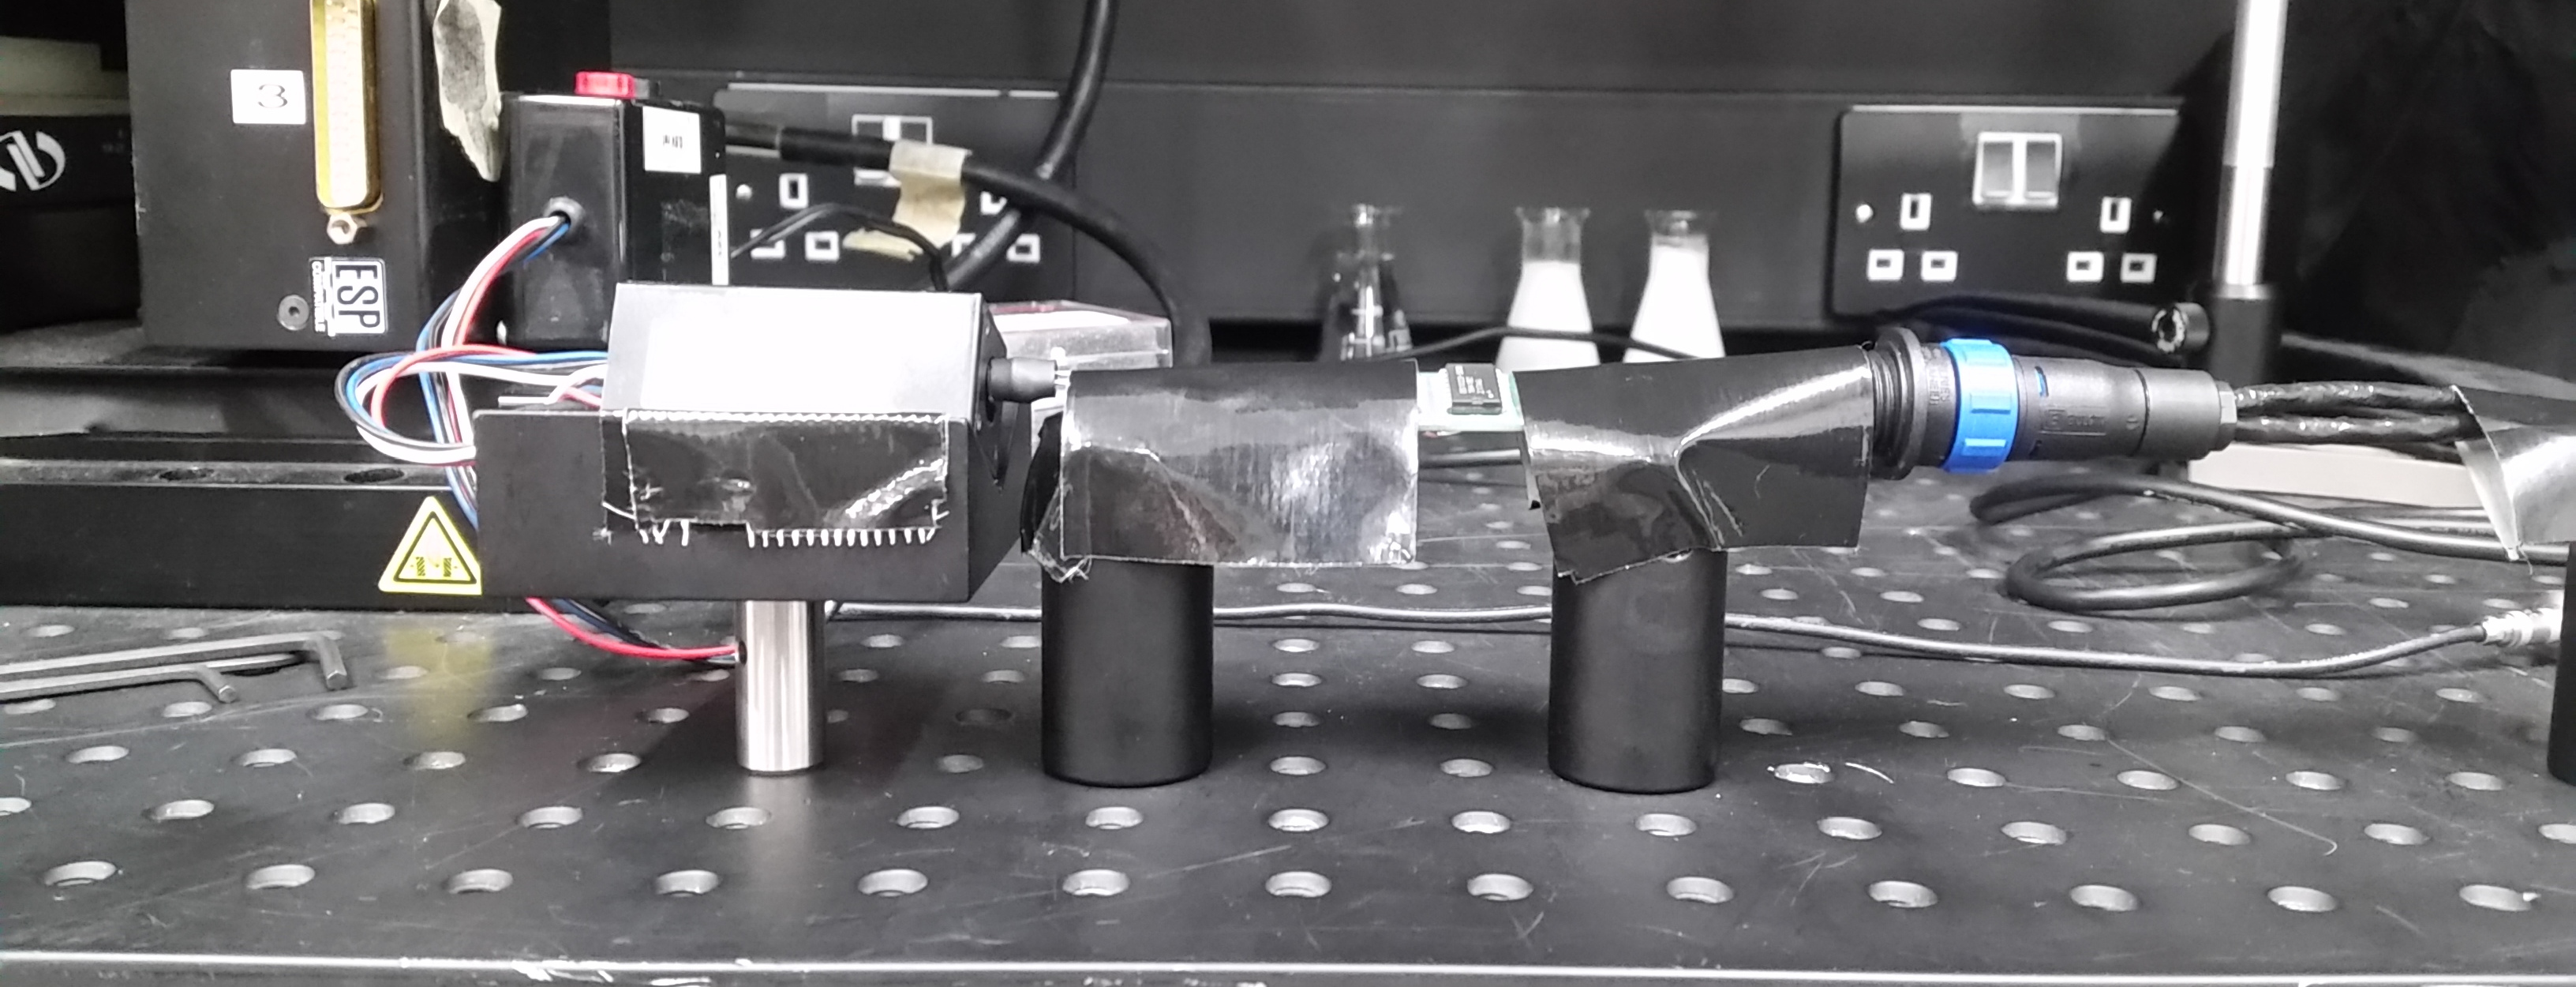
\includegraphics[width=\textwidth]{figures/PMTSetup.jpg}
    \caption{The experimental setup used to measure the intensity of the LED using the PMT.}
    \label{fig:PMTSetup}
\end{figure}

Eq.~\ref{eq:PMTPhotonCount} gives the number of photons seen by a PMT for a given pulse area. $A$ is the area of the pulse, $G$ is the gain of the PMT $R$ is the impedance of the oscilloscope ($50 \Omega$), $\epsilon_Q$ and $e$ is the charge of an electron. 

\begin{equation}
    N_\gamma = \frac{A}{G \cdot R \cdot \epsilon_Q \cdot e}
    \label{eq:PMTPhotonCount}
\end{equation}

The quantum efficiency of the PMT can be obtained from the radiant sensitivity ($R_s$) (shown in Figure~\ref{fig:pmtEfficiency}) using Eq.~\ref{eq:PMTQECalc}. At \SI{355}{nm} the quantum efficiency of the PMT is 0.4375. At \SI{420}{nm} the quantum efficiency of the PMT is 0.3591.

\begin{equation}
    \epsilon_Q = \frac{hc R_s}{e \lambda}
    \label{eq:PMTQECalc}
\end{equation}

\begin{figure}[H]
    \centering
    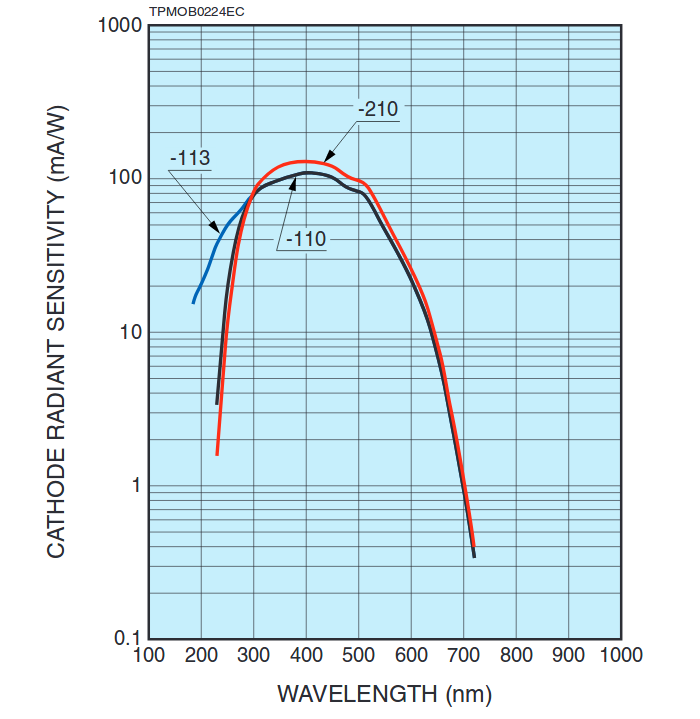
\includegraphics[width=0.5\textwidth]{figures/PMTEfficiency.png}
    \caption{The cathode radiant sensitivity as a function of wavelength~\cite{PMTDataSheet}.}
    \label{fig:pmtEfficiency}
\end{figure}


For a given voltage the gain of the PMT varies from PMT to PMT and needs to be calibrated for, several PMT measurements were measured at the same intensities as measurements made using the power meter (which provided the number of photons $N_\gamma$). By rearranging Eq.~\ref{eq:PMTPhotonCount} the gain can be calculated. 

Figure~\ref{fig:measuredGain} shows the measured value of the gain at varying intensities for the two wavelengths. The error bars are a combination of the error on the power meter measurements and the error on the average of approximately 10000 readings of the PMT area.

\begin{figure}[H]
    \centering
    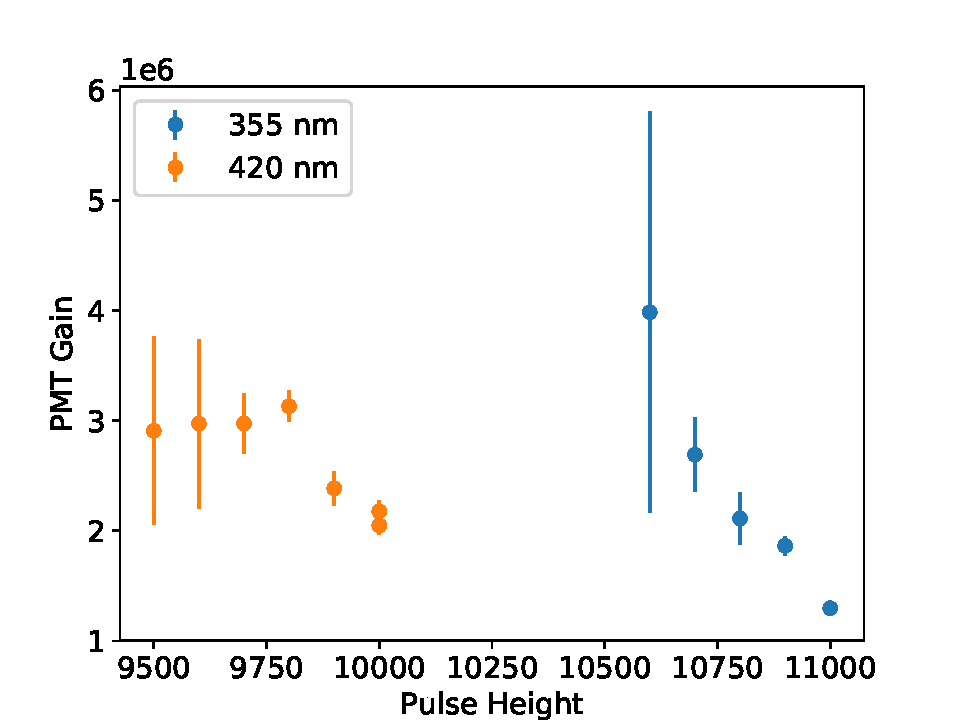
\includegraphics[width=0.6\textwidth]{figures/PMTGain.pdf}
    \caption{The measured PMT gain obtained by combining the power meter and PMT measurements.}
    \label{fig:measuredGain}
\end{figure}

The weighed average of the measurements of the gain gave an average value of \newline $1.9314 \pm 0.0368 \times 10^{6}$. The control voltage of the PMT was set to \SI{0.97}{V}, the measured gain agrees fairly well with the manufacturer supplied average gain shown in Figure~\ref{fig:PMTGainSpec}.

\begin{figure}[H]
    \centering
    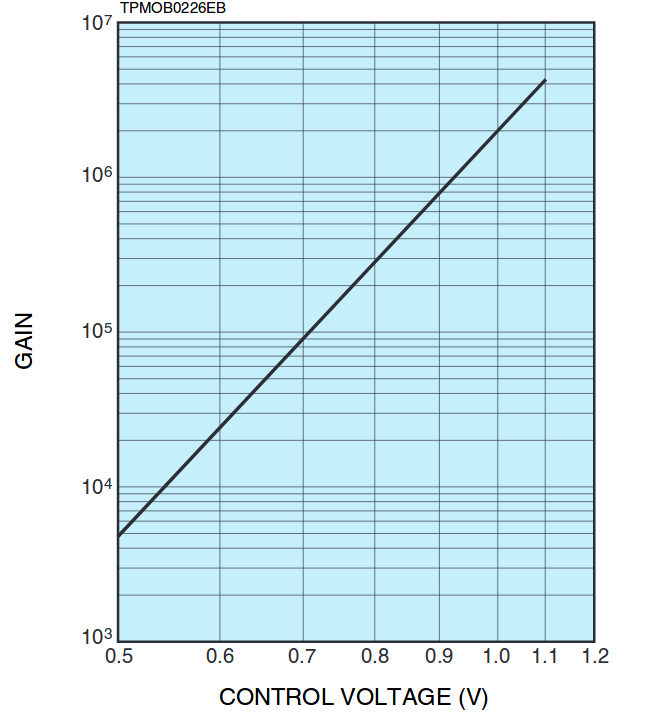
\includegraphics[width=0.6\textwidth]{figures/PMTGainSpec.png}
    \caption{The manufacturer specified average PMT gain as a function of control voltage~\cite{PMTDataSheet}.}
    \label{fig:PMTGainSpec}
\end{figure}

\subsection{Results}
Figure~\ref{fig:measurements420nm} shows the number of photons per pulse against the pulse height for the \SI{420}{nm} LED. The error bars on the power meter readings are just the RMS of the measurements made by the power meter. The error bars on the PMT are calculated by binning approximately 10000 PMT pulse areas and calculating the spread on the histogram which is then converted to the number of photons using Eq.~\ref{eq:PMTPhotonCount}, the weighed average value for the PMT gain was used. The driver is capable of reaching the \SI{e3}{photons } per pulse level.

\begin{figure}[H]
    \centering
    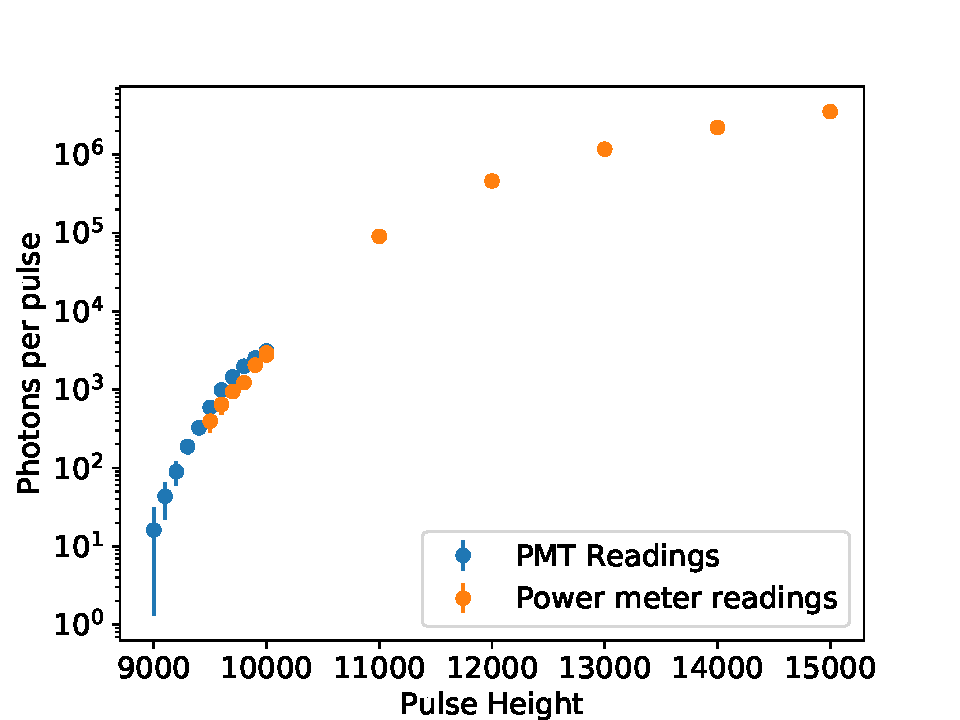
\includegraphics[width=0.8\textwidth]{figures/PhotonCounts420nm.pdf}
    \caption{The mean photons per pulse and error as a function of pulse height for the \SI{420}{nm} LED.}
    \label{fig:measurements420nm}
\end{figure}

The number of photons per pulse vs the pulse height for the \SI{355}{nm} LED is shown in Figure~\ref{fig:measurements355nm} , the error bars are calculated in the same way as the \SI{420}{nm} LED. With this LED the driver is also able to reach the \SI{e3}{photons } per pulse level.

\begin{figure}[H]
    \centering
    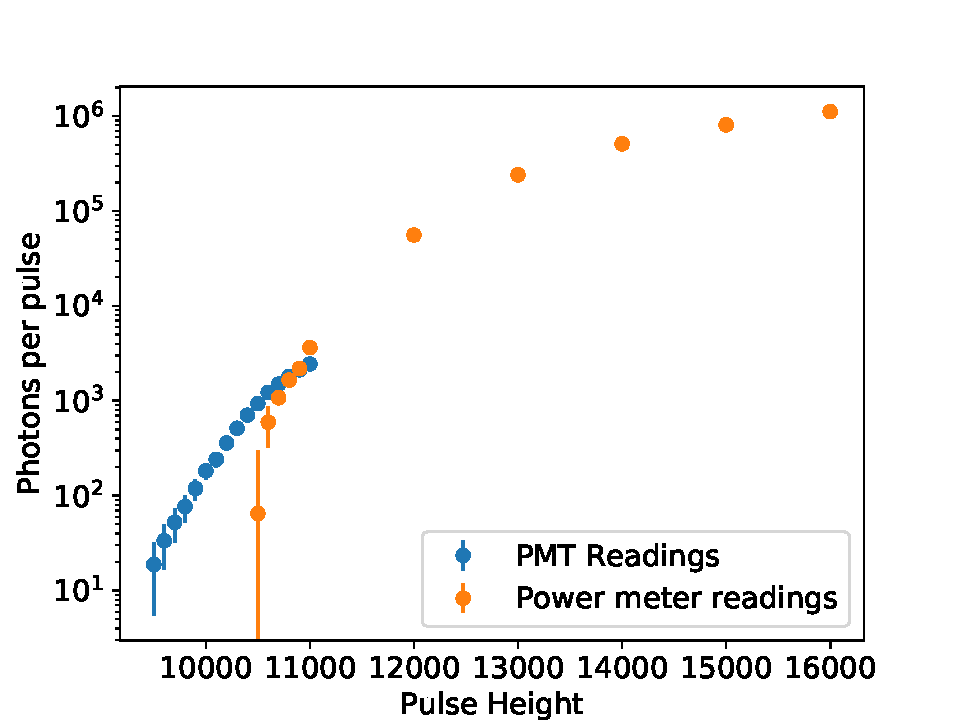
\includegraphics[width=0.8\textwidth]{figures/PhotonCounts355nm.pdf}
    \caption{The mean photons per pulse and error as a function of pulse height for the \SI{355}{nm} LED.}
    \label{fig:measurements355nm}
\end{figure}

\section{Conclusion}
This report describes the basic operation of the JSNS2 pulser system, a report into the intensity measurements of the driver when using both \SI{355}{nm} and \SI{420}{nm} LEDs is presented. For both wavelengths the driver is capable of reaching the \SI{e3}{photons } per pulse level required for operation within the detector.
\bibliographystyle{ieeetr}
\bibliography{references}


\end{document}
